\chapter{Построение модели решения задачи} 
Концепция сервиса опирается на интенсивное использование аппарата машинного обучения. Диаграммы процесса генерации \ref{fig:uml-inference} и обучения \ref{fig:uml-train} дают общее понимание процесса работы данного модуля. Далее будут рассмотрены как теоретические аспекты работы с моделями, так и результаты проведённых экспериментов.

\section{Цели и ограничения}
Основная цель данного модуля заключается в организации эффективного взаимодействия пользователя с аватаром через последовательный обмен сообщениями с последующей озвучкой сгенерированных текстовых сообщений. Ключевой особенностью является реалистичная имитация речевого поведения конкретного человека.

Описанная задача общения аватара с пользователем включает генерацию текста с учётом особенностей личности (persona-based text generation) в контексте домена обработки естественного языка (NLP). Дополнительно решается задача синтеза речи с имитацией голоса реального человека (voice imitation). Также в процессе формирования обучающего корпуса решается вспомогательная задача извлечения текста из аудио- и видеоматериалов (text extraction from audio/video).

Необходимо учитывать, что вычислительные ресурсы для генерации текста и аудио намного меньше, чем ресурсы, необходимые для обучения моделей. В целях демонстрации функционала, общение с аватаром будет осуществляться при помощи заранее обученных моделей, размещённых на бесплатных вычислительных мощностях таких сервисов, как Kaggle и Colab. Для демонстрации процесса обучения будут использованы модели небольших размеров с умеренными параметрами, чтобы снизить нагрузку на вычислительные мощности.


\section{Модуль генерации текста}
\subsection{Данные}
Формирование обучающего корпуса для аватара требует сбора и обработки значительных объёмов данных, характеризующих речевое поведение человека. Корпус включает три основных типа данных: текст, аудио и видео.

Каждый указанный формат поддерживается интерфейсом сервиса с возможностью загрузки популярных расширений файлов. Эти файлы преобразуются в исходные тексты, которые составляют первый тип данных в обучающем корпусе.

Вторым важным источником данных являются социальные сети, представляющие собой естественный источник коммуникации человека в современном мире. Данные социальных сетей имеют структуру вопрос-ответ и требуют персонального согласия пользователя на обработку. Реализована интеграция с мессенджером Telegram для автоматического сбора текстовых, аудио и видеосообщений из выбранных пользователем диалогов.

Итого, обучающий корпус включает исходные тексты, а также диалоговые сообщения из социальных сетей.

После получения данных в пайплайн обучения формируется структурированный датасет для дообучения модели генерации. Видеофайлы конвертируются в аудиофайлы формата WAV с помощью библиотеки moviepy. Затем начинается этап распознавания речи с помощью модели Whisper, аналогичный для полученных аудиофайлов, позволяющий получить текстовую транскрипцию с хорошей точностью.
На следующем шаге преобразованные и полученные текстовые файлы проходят стадию предобработки, в процессе которой удаляются лишние символы, технические вставки. Кроме того, слишком длинные предложения разбиваются на короткие, разбивая в основном на концах предложения, чтобы сохранить читаемость и связность.
В завершение все данные объединяются в единый текстовый корпус, готовый для запуска обучения.


\subsection{Выбор базовой модели}

Выбор языковой модели для задачи генерации текста в речевом стиле конкретного человека основывался на необходимости запуска обучения и генерации на бесплатных вычислительных ресурсах Kaggle, обеспечивая наилучший результат в рамках данных ограничений. Преимуществом использования платформы Kaggle для реализации пайплайнов является предоставление доступа к GPU ресурсам (NVIDIA Tesla P100 или T4), которых, несмотря на ограниченность, вполне достаточно для проведения экспериментов в научном проекте. Также немаловажным фактором в пользу использования данного облачного сервиса стало наличие официального API, который позволяет интегрировать использование вычислительных ресурсов в процесс обучения и генерации. 
На основании анализа научно-технической литературы и сравнительных оценок LLM было принято решение использовать модель из семейства Saiga. Основным критерием выбора послужили высокие результаты в бенчмарке PingPong, ориентированном на оценку в ролевых диалогах, одним из ключевых критериев которых является способность модели сохранять заданную роль. Наличие в обучающих корпусах этой серии данных, которые содержат разнообразные диалоговые и ролевые сценарии, что дополнительно подтверждает пригодность этих моделей для выбранной задачи.
Кроме того, линейка моделей Saiga включает в себя версии различной сложности и размеров, что позволило подобрать оптимальный вариант. Модель saiga\_mistral\_7b\_lora соответствует имеющимся ограничениям по вычислительным ресурсам, обладая хорошим уровнем качества генерации текста.
В рамках ограниченных ресурсов ее применение возможно благодаря технологии QLoRA, при которой модель заранее квантуется до 4-битного представления и фиксирует неизменными часть слоев, что позволяет значительно сократить объем занимаемой памяти при незначительной потере точности. Поэтому ее можно использовать на видеокартах с объёмом памяти 16 ГБ, которые доступны на платформе Kaggle.
Также в описании модели на платформе Hugging Face представлен сравнительный тест, где saiga\_mistral\_7b\_lora показала себя лучше, чем более крупная модель saiga2\_13b\_lora, основанная на архитектуре LLaMA 2, где при тесте 243 ответа были признаны лучшими, против 31 у последней и при 141 ничейном результате. При этом в серии моделей Saiga уступает более новой модели, основанной на архитектуре LLaMA 3, которая требует больших вычислительных ресурсов.


\subsection{Метрики}
На этапе выбора базовой модели для оценки качества генерации текста в речевом стиле конкретного человека главным элементом выступала human evaluation (человеческая экспертиза). Тем не менее учитывались следующие автоматические метрики:
\begin{itemize}
\item Perplexity — стандартная метрика, оценивающая степень «неопределённости» модели в предсказании следующего слова;
\item BLEU (Bilingual Evaluation Understudy) — оценивает сходство сгенерированного текста с эталонными образцами;
\item ROUGE (Recall-Oriented Understudy for Gisting Evaluation) — оценивает качество по наличию ключевых слов и выражений в сгенерированном тексте;
\end{itemize}
Однако численные метрики носили вспомогательный характер, а основное внимание уделялось качественной оценке результатов: насколько текст реалистичен, естественен, и соответствует интонациям и стилевым особенностям пользователя.


\subsection{Токенизация}
Для токенизации текста используется алгоритм Byte-Pair Encoding (BPE), который позволяет эффективно работать с большим словарём слов, сохраняя баланс между объёмом данных и скоростью обработки. Использование BPE помогает эффективно представлять редкие слова и специализированные термины, что особенно важно для персонализированной генерации текста.

\subsection{Обучение}

Процесс дообучения модели реализован в рамках чистой архитектуры, что обеспечило высокую модульность и отделение бизнес-логики от технических деталей. Все ключевые компоненты пайплайна — загрузка данных, проверка ресурсов, запуск обучения и сохранение результатов — организованы в виде изолированных модулей с интерфейсами. Такой подход позволяет быстро адаптировать архитектуру под новые требования в условиях стремительного развития LLM.
Дообучение может запускаться как на локальной машине, так и на бесплатных вычислительных ресурсах Kaggle. Выбор режима настраивается в конфигурационном файле. По умолчанию создается и запускается Kaggle-ноутбук с предварительно загруженным датасетом. Изменением одной переменной можно переключиться на локальное выполнение, что особенно полезно в условиях ограниченного доступа к аппаратным ресурсам.
Запуск пайплайна осуществляется в отдельном процессе, что позволяет оставлять сервис в активном состоянии. Однако новые запросы на обучение игнорируются, пока работает хотя бы одна задача обучения.
Конечная модель сохраняется в S3-хранилище, откуда потом используется для пайплайна генерации текста.

\subsection{Генерация текста}
Генерация текста построена по аналогичной модульной логике: в зависимости от настроек может использоваться локальный или удаленный режим. Ранее дообученная модель загружается из облачного хранилища для генерации ответа. Благодаря изолированной структуре, интеграция новой модели для генерации требует минимальных изменений — достаточно заменить соответствующий компонент, не затрагивая остальную часть пайплайна.
Этот подход сохраняет гибкость системы и упрощает ее масштабирование при работе с различными моделями и окружениями.

\section{Модуль генерации звука}
Для синтеза речи используется короткий аудиофрагмент продолжительностью порядка 15 секунд,  
достаточный для точной имитации тембра и артикуляции голоса пользователя.
Прикладная направленность задача звукового модуля задаёт акцент на практической пригодности решения и рациональном  
использовании вычислительных ресурсов, без разработки принципиально новых архитектур.

\subsection{Выбор базовой модели}

При выборе модели для синтеза речи ключевым критерием была способность точно воспроизводить
голос пользователя на основе короткого аудиофрагмента. В процессе исследования различных
решений, доступных на платформах GitHub и Hugging Face, было рассмотрено несколько подходов.

Одним из первых протестированных решений стала реализация \textbf{Real-Time Voice Cloning}
от CorentinJ \cite{jemine2019voicecloning}. Эта модель демонстрирует хорошие результаты в задачах
клонирования голоса и может работать в реальном времени. Однако, как отмечает сам автор,
существуют более современные и качественные решения в области синтеза речи. В частности,
он рекомендует обратить внимание на проекты, представленные на \textbf{paperswithcode}, а
также на такие решения, как \textbf{CoquiTTS} \cite{coquitts} и \textbf{MetaVoice-1B} \cite{metavoice2024}.

Следует отметить, что, несмотря на то, что проект \textbf{CoquiTTS} более не поддерживается его первоначальной 
командой разработчиков, он продолжает развиваться силами сообщества и остаётся актуальным благодаря регулярным 
обновлениям и исправлениям. В ходе тестирования CoquiTTS продемонстрировал стабильную работу, хорошую адаптацию 
к русскому языку и возможность кастомизации тембра речи, что сделало его оптимальным выбором в качестве 
основной модели синтеза речи в рамках проекта.

Параллельно с этим была предпринята попытка интеграции более актуальной архитектуры \textbf{LLASA} (LLaMA-based Speech Synthesis) \cite{ye2025llasa}. Эти модели представляют собой современные
решения в области синтеза речи, основанные на архитектуре LLaMA и интегрированные с кодеком
XCodec2. Особенностью моделей LLaSA является их способность к высококачественному синтезу речи
и поддержка многозадачного обучения.

Семейство LLaSA включает модели с различным количеством параметров: 1, 3 и 8 миллиардов.
Однако полное переобучение даже минимальной версии \textbf{HKUSTAudio/Llasa-1B} требует
значительных вычислительных ресурсов и большого объёма обучающих данных, что выходит за
рамки доступных возможностей. Поэтому было принято решение использовать предобученную
версию \textbf{Llasa-1B-Multilingual}, обладающую следующими преимуществами:

\begin{itemize}
  \item Высокая естественность синтезируемой речи «из коробки» и унифицированная
        BPE-токенизация без необходимости в G2P-преобразовании.
  \item Компактный объём (около 1 миллиарда параметров), позволяющий проводить тонкую
        настройку модели на одной GPU с объёмом памяти 24 GB.
\end{itemize}

Основным недостатком выбранной модели является отсутствие русского корпуса в изначальной
предобученной выборке, что требует дополнительного дообучения на соответствующих данных.

\subsection{Подготовка данных}

Для обучения и валидации использован открытый корпус  
\textbf{Russian Open Speech To Text}. Из него сформированы  
тематические подкорпуса суммарным объёмом около 460 GB WAV, охватывающие  
бытовую речь, подкасты, лекции, радиопередачи и ролики YouTube. Подготовка  
аудио-текстовых пар включала четыре этапа. Сначала исходные записи проходили  
базовую процедуру нормализацию: обрезку тишины, выравнивание уровня громкости и  
преобразование частоты дискретизации к 16 кГц. Затем текст каждой реплики  
токенизировался встроенной BPE-моделью LLaSA, обеспечивая единый словарь для  
всех языков. Далее аудиодорожки дискретизировались в компактные токены  
кодеком XCodec2. Наконец, пары «текст–звук» сохранялись в формате  
\textbf{Hugging Face Datasets}, что позволяло без дополнительной конвертации  
использовать их в пайплайне дообучения и сохранить больше вычислительных мощностей 
для переобучения модели, а также сохранить целостность сформированных датасетов. 

\begin{table}[h!]
  \centering
  \begin{tabular}{|l|c|c|}
    \hline
    \textbf{Префикс} & \textbf{Объём, GB} \\ 
    \hline
    asr\_calls\_2\_val                       & 2     \\
    buriy\_audiobooks\_2\_val                & 1     \\
    public\_youtube700\_val                  & 2     \\ 
    public\_lecture\_1                       & 0.7   \\
    public\_series\_1                        & 1.9   \\
    asr\_public\_stories\_1                  & 4.1   \\
    asr\_public\_stories\_2                  & 9     \\
    asr\_public\_phone\_calls\_1             & 22.7  \\
    public\_youtube1120\_hq                  & 31    \\
    asr\_public\_phone\_calls\_2             & 66    \\
    public\_youtube700                       & 75    \\
    tts\_russian\_addresses\_rhvoice\_4voices& 80.9  \\
    radio\_2                                 & 154   \\
    public\_youtube1120                      & 237   \\
    \hline
  \end{tabular}
  \caption{Подкорпуса Russian Open Speech To Text, отобранные для дообучения}
  \label{tab:ru_splits}
\end{table}


\subsection{Гиперпараметры дообучения модели}

Для успешного переноса модели на русский язык важное значение имеет выбор гиперпараметров обучения.  
Корректная настройка параметров оптимизации, регуляризации и аппаратного обеспечения обеспечивает  
достижение стабильной сходимости и приемлемого качества генерации. В таблице \ref{tab:ft_hparams}  
приведены ключевые гиперпараметры, использованные в ходе финального цикла дообучения модели.

\begin{table}[h!]
\centering
  \begin{tabular}{|c|c|}
    \hline
    Параметр & Значение \\
    \hline
    Модель & \texttt{HKUSTAudio/Llasa-1B-Multilingual} \\
    \hline
    Тип данных & \texttt{bfloat16}, Flash-Attention 2 \\
    \hline
    Оптимизатор & 8-bit Adam (bitsandbytes) \\
    \hline
    Learning Rate & $5\!\cdot\!10^{-5}$ (cosine schedule) \\
    \hline
    Warmup Ratio & 0.03 \\
    \hline
    Weight Decay & 0.01 \\
    \hline
    Batch Size & 16 аудио-сегментов \\
    \hline
    Эпох & 3 \\
    \hline
    Gradient Acc. & 1 \\
    \hline
    Аппаратная база & одна NVIDIA A100 40 GB \\ 
    \hline
  \end{tabular}
  \caption{Ключевые гиперпараметры дообучения}
  \label{tab:ft_hparams}
\end{table}

\subsection{Процесс дообучения и отслеживание параметров}

Эффективное управление процессом обучения требует постоянного мониторинга показателей, таких как  
функция потерь и другие вспомогательные метрики. Для обеспечения прозрачности экспериментов,  
удобства визуализации динамики и последующего анализа была выбрана платформа Weights \& Biases.  
Данная платформа позволяет фиксировать следующие параметры и характеристики обучения:

\begin{itemize}
  \item графики функции потерь на обучении и валидации;  
  \item изменения значений MOS после завершения дообучения;  
  \item контрольные аудио-сэмплы, позволяющие оценить промежуточные результаты;  
  \item хэш коммита и конфигурацию гиперпараметров для воспроизводимости экспериментов.  
\end{itemize}

На рисунках \ref{fig:loss_curve1} и \ref{fig:loss_curve2} представлены примеры визуализации 
основных параметров, т.е. функции потерь в данном случае, полученные при дообучении модели.

\begin{figure}[h]
  \centering
  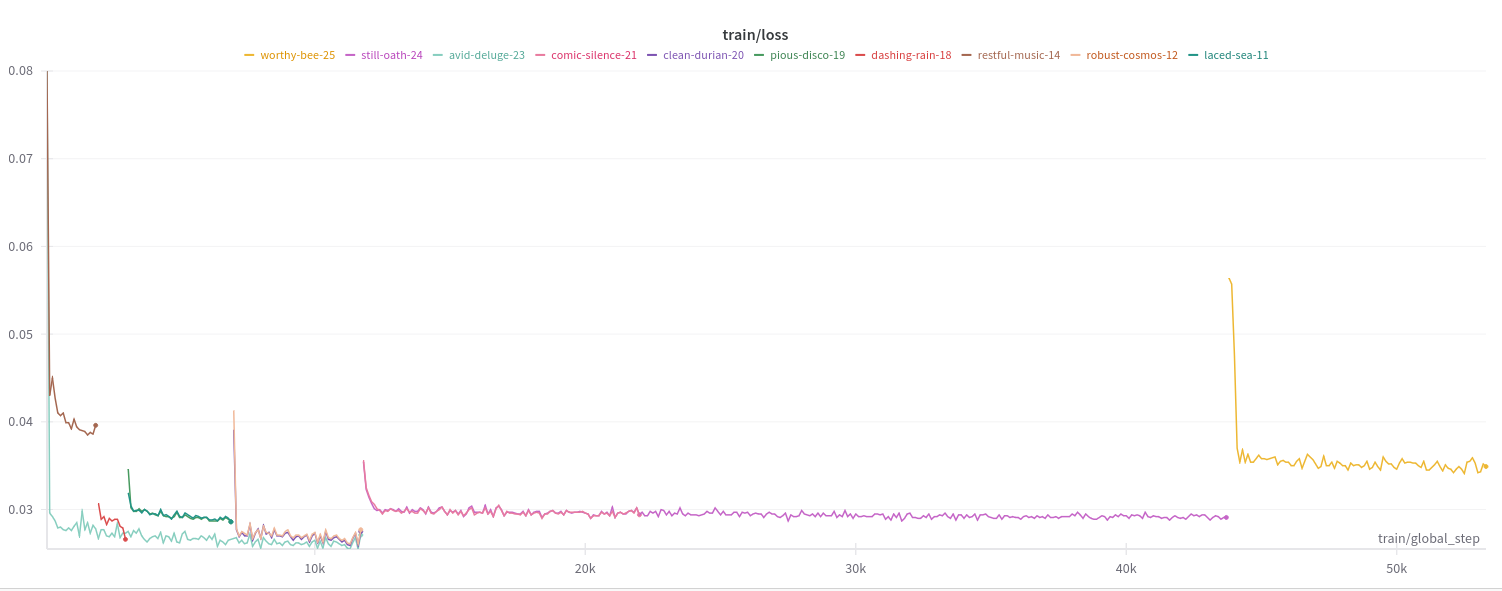
\includegraphics[width=0.9\textwidth]{images/wandb-train-loss.png}
  \caption{Динамика функции потерь на обучении}
  \label{fig:loss_curve1}
\end{figure}

\begin{figure}[h]
  \centering
  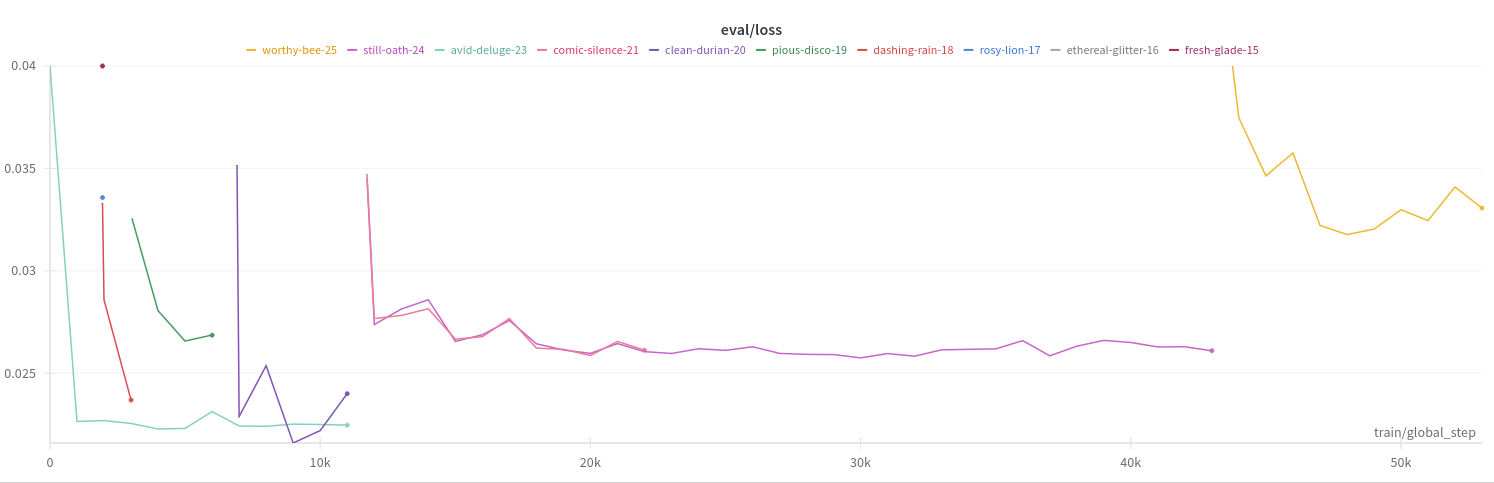
\includegraphics[width=0.9\textwidth]{images/wandb-eval-loss.png}
  \caption{Динамика функции потерь на валидации}
  \label{fig:loss_curve2}
\end{figure}


\subsection{Оценка качества генерации и используемые метрики}

Итоговая оценка качества синтезированной речи представляет собой важнейший этап, подтверждающий практическую пригодность разработанной модели. Особое значение в этом контексте имеет субъективное восприятие конечного пользователя — естественность, эмоциональность и узнаваемость голоса. Для финальной проверки качества планировалось использовать метрику \textbf{Mean Opinion Score (MOS)}, которая широко применяется в задачах оценки качества синтетической речи.

Методика предполагала генерацию набора из 20 «слепых» аудио-сэмплов на фиксированном контрольном тексте, с последующим прослушиванием и оценкой каждого сэмпла группой из пяти независимых слушателей по шкале от 1 до 5. На основе этих оценок рассчитывались среднее значение и дисперсия MOS, что позволило бы количественно зафиксировать степень естественности и узнаваемости полученной речи.

Однако на практике полная реализация данного подхода оказалась невозможной из-за ограниченных вычислительных ресурсов. Провести полноценное обучение модели в запланированном объеме не удалось — была реализована лишь часть обучающих итераций, в результате чего качество сгенерированной речи оставалось далеко от ожидаемого. В таких условиях применение MOS стало неинформативным: оценки слушателей варьировались случайным образом, не отражая объективных различий в качестве, а результирующие значения средней оценки не позволяли сделать достоверные выводы. Таким образом, при текущем уровне реализации метрика MOS оказалась неприменимой и не может использоваться для формальной оценки итогового качества.

В связи с вышеописанными ограничениями, для получения качественных аудио-сэмплов было принято решение использовать готовую модель из библиотеки \textbf{Coqui TTS}.
